
\documentclass{article}
\usepackage{graphicx}
\title{Ch 121a Proposal}
\author{Patryk Kozlowski}
\date{\today}
\begin{document}
\section{Perovskites}
\subsection{Structure}
The ideal perovskite stucture is ABO$_3$, where A is a large cation, B is a smaller cation, and O is an oxygen anion. The B cation is typically a transition metal, and the A cation is typically an alkali metal or alkaline earth metal. The structure is face-centered cubic, with the B cation at the center of the cube, the A cation at the corners of the cube, and the O anion at the center of each face of the cube. The structure is shown in Figure 1.
\begin{figure}
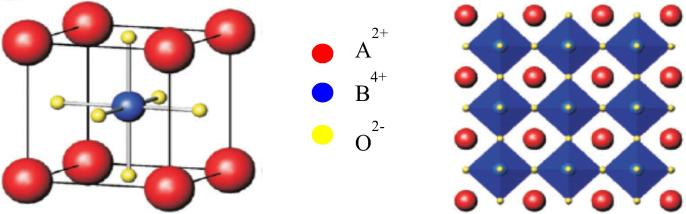
\includegraphics[width=\linewidth]{perovskite.png}
\caption{The ideal face-centered cubic perovskite structure. \cite{assirey2019perovskite}}
\label{fig:perovskite}
\end{figure}
\subsection{Applications}
Perovskites have shown potential as efficient heterogeneous catalysts that are cheap and easy to synthesize. Additionally, the structure of perovskites allows for a wide range of substituting and doping, allowing to tailor their properties to better target applications \cite{royer2014perovskites}. They show promise in Catalytic NO Decomposition, catalytic NO Reduction, Catalytic N2O Decomposition, Catalytic Complete Oxidation of CO and CH4, Catalytic Oxidative Reforming of Hydrocarbon, Soot Oxidation, and Catalytic Combustion of Volatile Organic Compounds (VOCs) to name a few. \cite{zhu2014perovskite}
\section{Objectives}
I will be using VASP to compute surface energies of perovskites, first using DFT and then  potentially using wavefuntion-based methods like HF/MP2. I want to compute surface energies for the La series of perovskites; starting with LaMnO3, LaFeO3, and LaCoO3. I think this would be interesting because the transition metal cation is changing across the series, and I would like to see how this affects the surface energies. I will compare my results to experimental/computational data from the literature (material project).
\section{Method}
% \subsection{Find experimental data for comparison}
% Look through Materials Project? Not sure how to select the data I want.
\subsection{Perform DFT calculations}
\subsubsection{Choice of DFT functional}
PBE-D3
% \subsubsection{Basis choice}
% Is this needed for VASP?
% \subsubsection{Choice of k-point mesh}
% \subsubsection{choice of surface}
% is this needed here? For example, for Pt we chose the (111) surface.
\subsection{Perform HF/MP2 or hybrid-DFT calculations}
This might be a good continuation into Ch121b. I will start on DFT now in Ch121a, and then move on to HF in Ch121b.
\bibliographystyle{unsrt}
\bibliography{citations}
\end{document}
